
\begin{figure*}[ht!]
\centering
\begin{minipage}[t]{.49\textwidth}
\centering
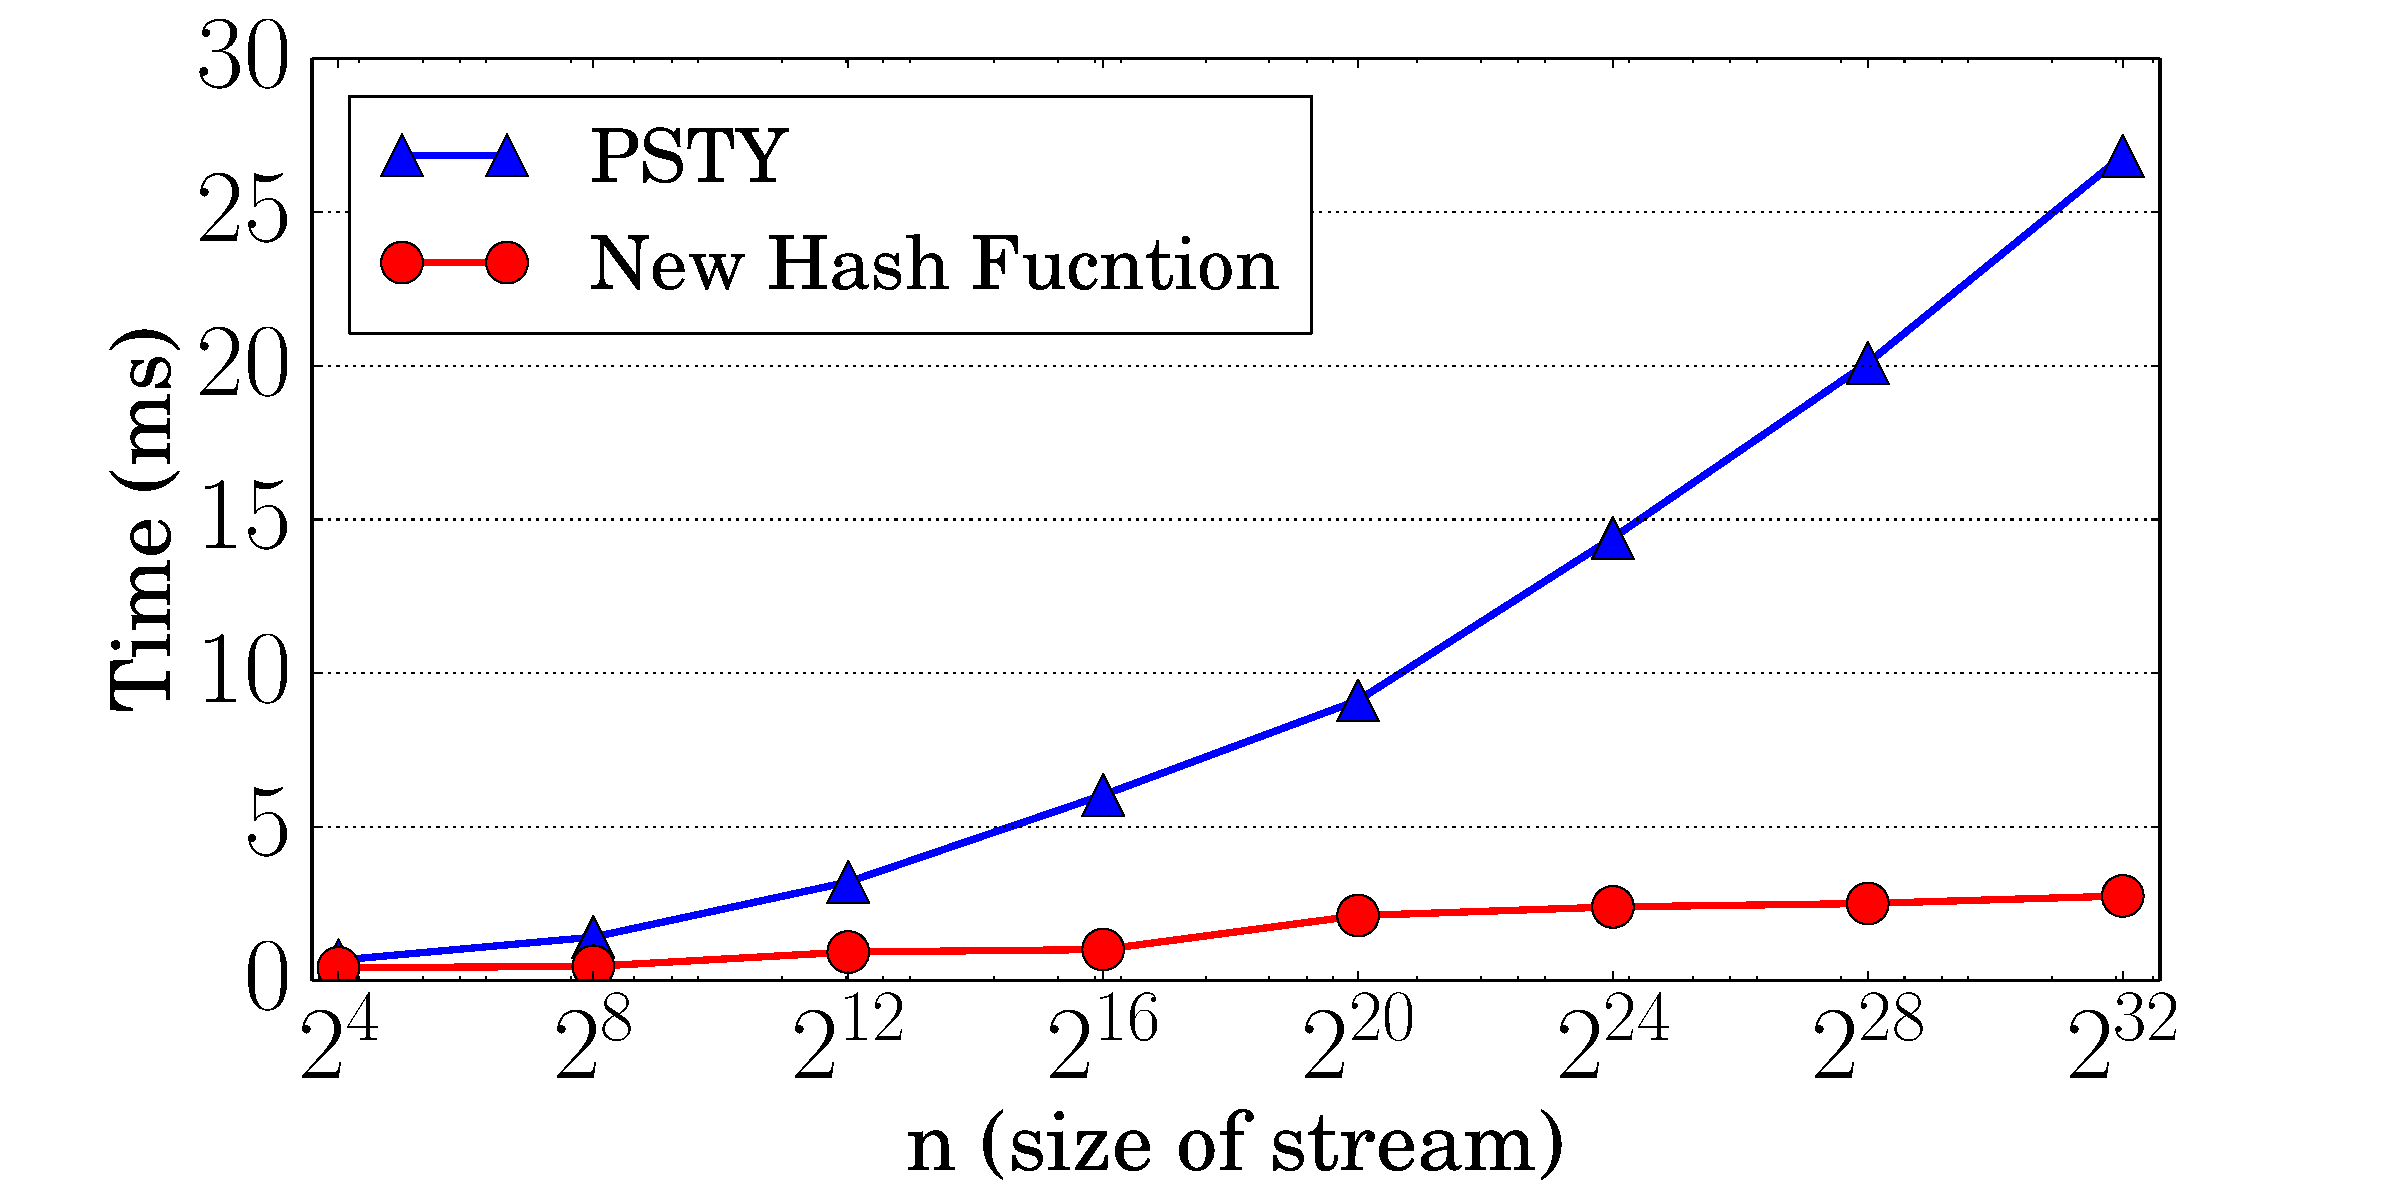
\includegraphics[scale = 0.23]{fig/hashtime.pdf}
\caption{Running time of the hash functions. In the $x$ axis, we present the size $n$ of the stream in $\log$ scale. The new hash function $h_{new}$ is $1.6\times$ faster when $n = 2^4$, and $9.8\times$ faster when $n=2^{32}$, than $h_{old}$.}\label{hashtime}
\end{minipage}\hfill
\begin{minipage}[t]{.49\textwidth}
\centering
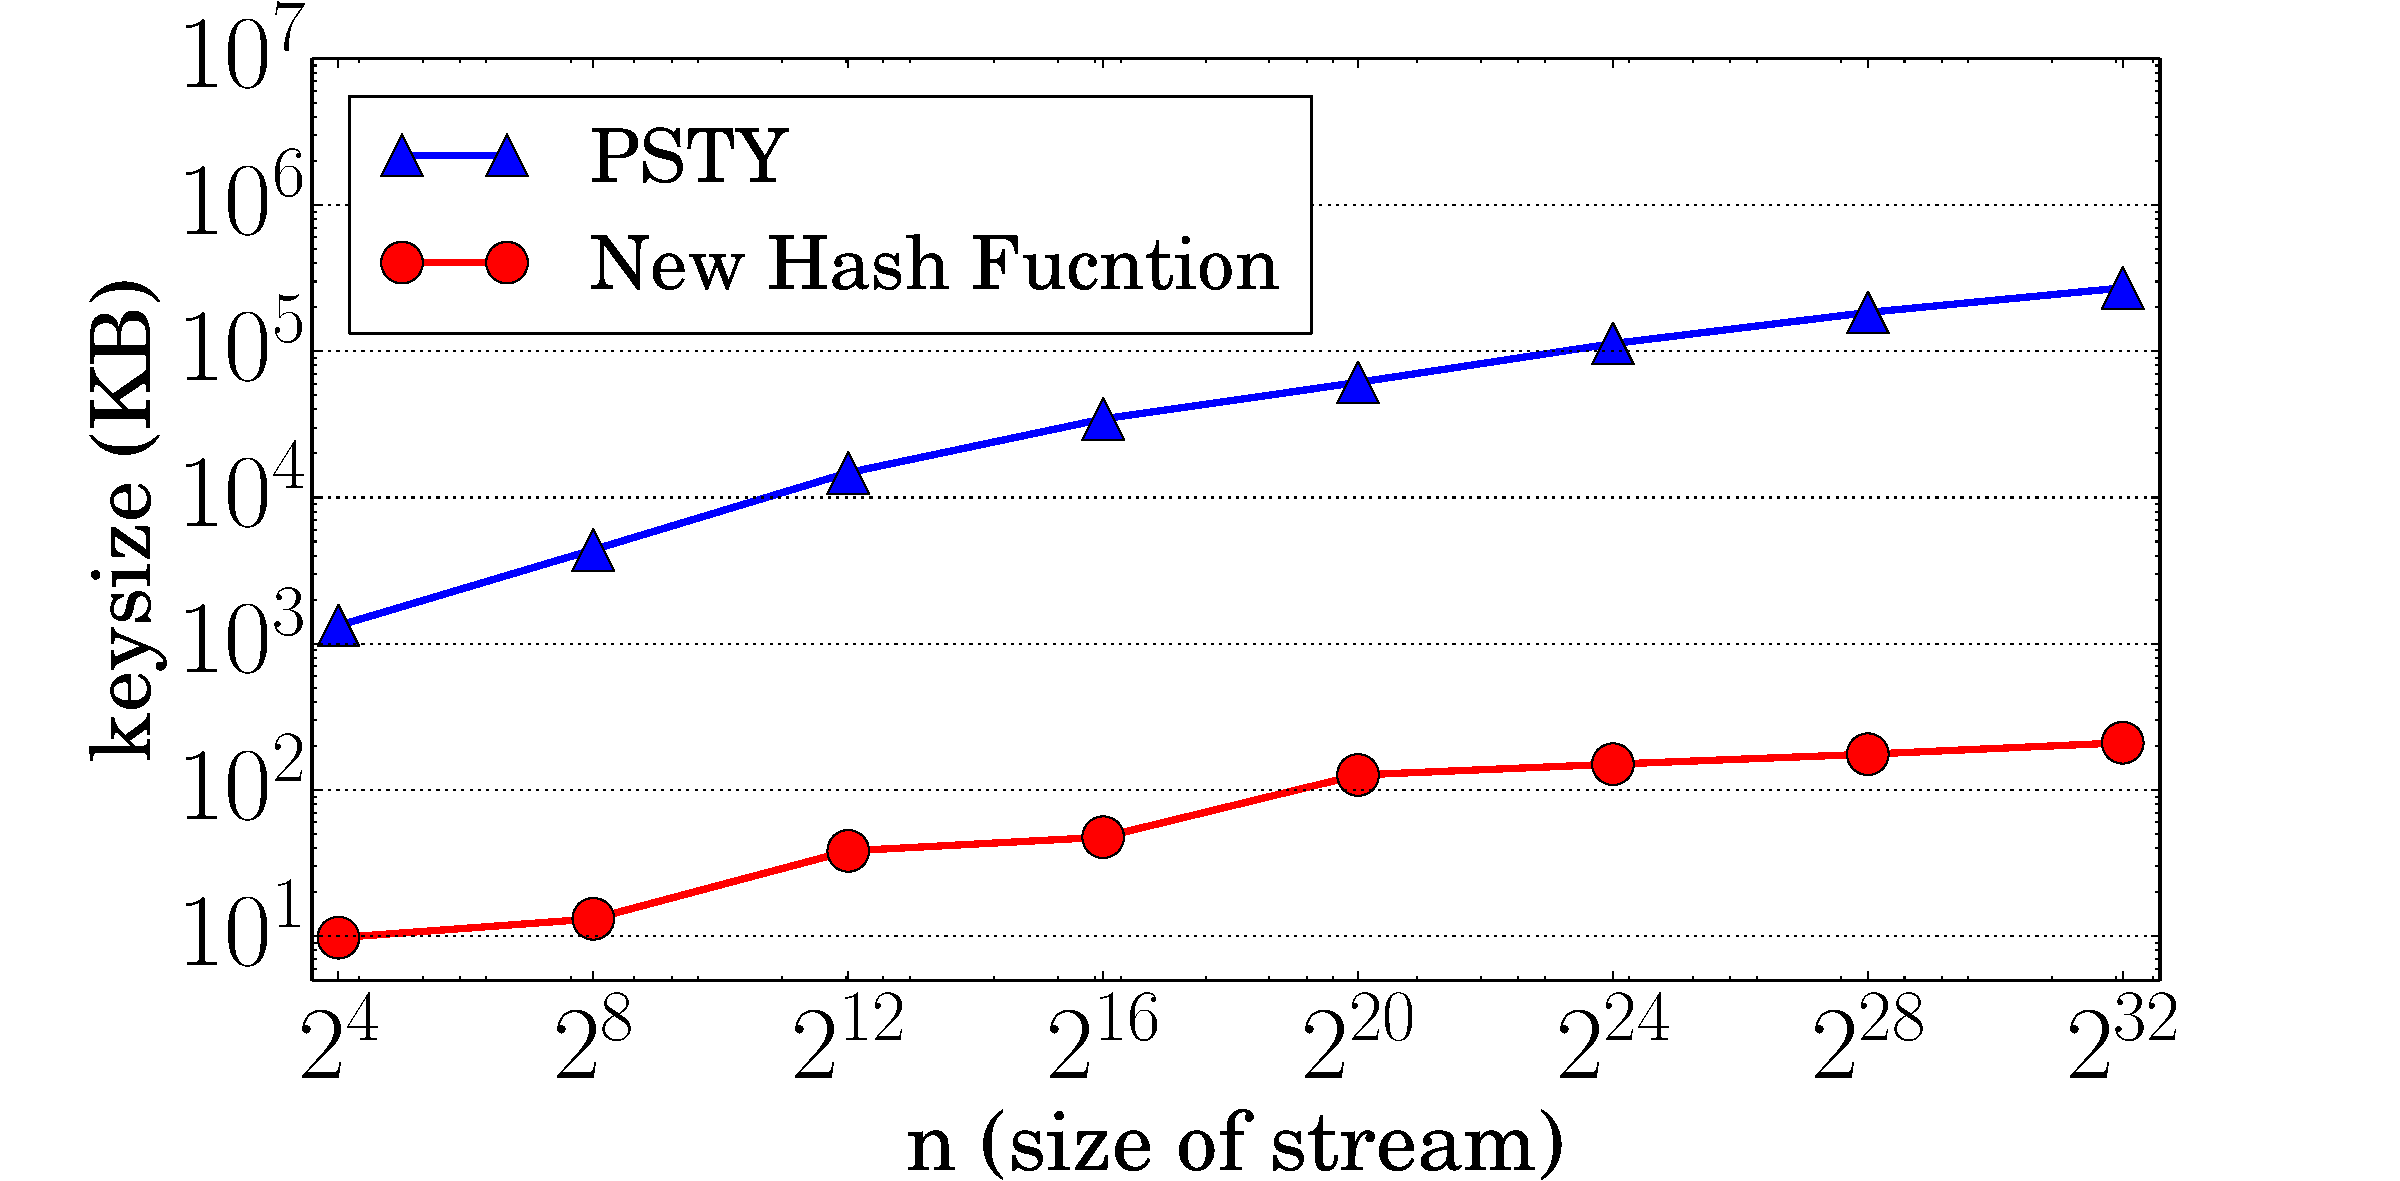
\includegraphics[scale = 0.23]{fig/keysize.pdf}
\caption{Key size of the hash functions. In the $x$ axis, we present the size $n$ of the stream and in the $y$ axis we show the key size in KB. The figure is in $\log-\log$ scale. The key size of $h_{new}$ is only 0.73\% when $n=2^4$, and 0.077\% when $n=2^{32}$, of $h_{old}$.}\label{keysize}
\end{minipage}\hfill
\end{figure*}

\section{Optimization}\label{modification}

%\babis{the algorithm is not correct, please change according to our discussions}
%\babis{For probability, use $\Pr[x=5]$}
In this section, we introduce a modified labeling function for the PSTY scheme~\cite{DBLP:conf/eurocrypt/PapamanthouSTY13} that reduces the space complexity by a factor of $\sqrt{n}$, except with negligible probability. Since this labeling function does not rely on any properties of the hash function, the modification also applies to any instantiations with the same projection function, inverse projection function and the $\gamma$ function introduced in section~\ref{instantiation}.

\ignore{
\begin{defn}[Modified Labeling]\label{modified_label}
Let $T_{\mathcal{C}}$ be a structured binary tree, where $\mathcal{C} = [c_{0}, c_{1}, \dots, c_{M-1}]$. For every node $w \in T_{\mathcal{C}}$ we define its label $\lambda(w) = \sum_{v\in \textsf{\emph{range}}(w)} c_v\cdot \delta_{w}(v) \bullet \textsf{\small \emph{rand()}}$, where $\delta_{w}(v)$ is the unit update defined by Definition~\ref{delta}, \textsf{\small \emph{rand()}} outputs a random vector from $\{-1,1\}^{k \cdot t}$ and $\bullet$ is the scalar dot product.
\end{defn}

}

\begin{defn}[Modified Labeling]\label{modified_label}
Let $T_{\mathcal{C}}$ be a structured binary tree, where $\mathcal{C} = [c_{0}, c_{1}, \dots, c_{M-1}]$. For every node $w \in T_{\mathcal{C}}$ we define its label $\lambda(w) = \sum_{v\in \textsf{\emph{range}}(w)} c_v\cdot \delta_{w}(v) \bullet \emph{\textsf{\small rand()}}$, where $\delta_{w}(v)$ is the unit update defined by Definition~\ref{delta}, $\emph{\textsf{\small rand()}}$ outputs a random bit from $\{-1,1\}$ and $\bullet$ is the scalar product.
\end{defn}

The random function \textsf{\small rand()} can be generated and retrieved by a pseudorandom generator with a public key. Given the $\gamma$ function as Equation~\ref{gamma1}, it is obvious that $\mathcal{L}_w(v) = c_v\cdot \delta_w(v)$. Next, we prove the size of the labels will be reduced to $O(\sqrt{n}) $ by this optimization.



\begin{lemma}\label{lemma_iid}
Assume elements in $\mathcal{C} = [c_{0}, c_{1}, \dots, c_{M-1}]$ are independent and identically distributed (i.i.d.), with mean $\mu$ and variance $\sigma^2$. For a node $w$ and a leaf $v\in\textsf{\emph{range}}(w)$, Let $\mathcal{P}_w(v)= c_{v} \cdot \delta_{w}(v) \bullet \textsf{\small \emph{rand()}} = [p_{1}, p_{2}, \dots, p_{{k \cdot t}}]$. Let $\delta_{w}(v) =[\delta_{1}, \delta_{2}, \dots, \delta_{k \cdot t}]$. For $1 \leq j \leq k \cdot t$, we have
\[  
  \{\begin{array}{l l}
    p_{j}=0 & \quad \text{if $\delta_{j}=0$;}\\
    p_{j} \emph{ is }i.i.d.\emph{ with mean 0 and variance } \mu^2+\sigma^2 & \quad \text{if $\delta_{j}=1$.}
  \end{array} 
  \]
\end{lemma}

\begin{proof}
For $1\le j\le k\cdot t$, $\delta_j$ is a deterministic binary value by Definition~\ref{delta}. In the first case, $p_{j}=0$ is trivially true when $\delta_{j}=0$. We consider the second case when $\delta_{j}=1$. Since \textsf{\small rand()} returns $1(-1)$ with $1/2$ probability independently and all elements in $\mathcal{C}$ are independent and identically distributed, we have the probability mass function of $p_{j}$ as the follows:
$$f_{p_j}(x)=
\begin{cases}
\frac{1}{2}f_{C}(x)& x>0\\
\frac{1}{2}f_{C}(-x)& x<0
\end{cases},$$
where $f_{C}$ is the probability mass function of elements in $C$. Since the distribution of $C$ has mean $\mu$ and variance $\sigma^{2}$, we have $\mu_{p_j} = 0$ and $\sigma_{p_j}^2 = \mu^2+\sigma^2$.
\end{proof}



\begin{lemma}\label{lemma_gaussian}
Let the label of the root $\lambda(r) =[\lambda_{1}, \lambda_{2}, \dots, \lambda_{k \cdot t}]$. For $1\le j\le k\cdot t$, let $n_j$ be the total number of leaves with nonzero $p_j$ defined in Lemma~\ref{lemma_iid}. Then, $\frac{\lambda_{j}}{\sqrt{n_{j}}}$ follows Gaussian distribution $N(0, \mu^2+\sigma^2)$ as $n_{j} \to \infty$.
\end{lemma}



\begin{proof}
Following directly from the Definition~\ref{modified_label} and Lemma~\ref{lemma_iid}, $\lambda_{j}$ is the summation of $n_{j}$ i.i.d random variables.  By the \textbf{Central Limit Theorem}, $\frac{\lambda_{j}}{\sqrt{n_{j}}} \sim N(0, \mu^2+\sigma^2)$ as $n_{j} \to \infty$. 


\end{proof}

\begin{lemma}\label{lemma_bound}
Let \textbf{\emph{X}} be a Gaussian distribution with mean 0 and variance $\sigma^2$, then $\Pr[\textbf{\emph{X}}>t] < \frac{1}{\sqrt{2\pi} \sigma t}e^{-\frac{t^2}{2\sigma^2}}$. 
\end{lemma}

\begin{proof}
By definition, $\Pr[\textbf{X}>t] = \int_{t}^{\infty} \frac{1}{\sqrt{2\pi} \sigma} e^{-\frac{x^2}{2\sigma^2}} dx$. We can bound the above expression by the following: $$\int_{t}^{\infty} \frac{1}{\sqrt{2\pi} \sigma} e^{-\frac{x^2}{2\sigma^2}} dx < \frac{1}{\sqrt{2\pi} \sigma t} \int_{t}^{\infty}xe^{-\frac{x^2}{2\sigma^2}} dx = \frac{1}{\sqrt{2\pi} \sigma t}e^{-\frac{t^2}{2\sigma^2}}$$. 
\end{proof}



\begin{theorem}
Let $w$ be any node in a generalized hash tree. Every element $\lambda_{j}$ of its modified labeling $\lambda(w)$ by Definition~\ref{modified_label} is in $[-t\sqrt{n}, t\sqrt{n}]$ for some constant $t$, except with negligible probability \textsf{\small \emph{neg($t$)}}.
\end{theorem}


\begin{proof}
By Lemma~\ref{lemma_gaussian}, $\frac{\lambda_{j}}{\sqrt{n_{j}}} \sim N(0, \mu^2+\sigma^2)$. Therefore,

\begingroup\makeatletter\def\f@size{9}\check@mathfonts
\def\maketag@@@#1{\hbox{\m@th\large\normalfont#1}}%
\begin{align*}
&\Pr[|\lambda_{j}| > t\sqrt{n}] < \Pr[|\lambda_{j}| > t\sqrt{n_{j}}] \nonumber \text{\ \ (Lemma~\ref{lemma_gaussian})}\\
&= \Pr[|\frac{\lambda_{j}}{\sqrt{n_{j}}}| > t] \\
&= 2\Pr[\frac{\lambda_{j}}{\sqrt{n_{j}}} > t] \\
&< 2\times \frac{1}{\sqrt{2\pi(\mu^2+\sigma^2)}  t}e^{-\frac{t^2}{2(\mu^2+\sigma^2)}} \nonumber \text{\ \ (Lemma~\ref{lemma_bound})},
\end{align*}\endgroup
which is negligible \textsf{\small{neg($t$)}}.

\end{proof}

